\documentclass[a4paper,11pt]{article}
% Use ctrl + alt + V to view live pdf

% Packages
\usepackage[utf8]{inputenc} % For encoding
\usepackage[T1]{fontenc} % Better handling of accented characters and hyphenation
\usepackage{microtype} % Improves spacing and justification
\usepackage{amsmath, amssymb} % For equations and symbols
\usepackage{graphicx} % For including graphics/images
\usepackage{caption} % For customizing figure and table captions
\usepackage{subcaption} % For subfigures and subcaptions
\usepackage{float} % For fixing figure and table positions
\usepackage{booktabs} % For professional-looking tables
\usepackage{siunitx} % For consistent typesetting of units and numbers
\usepackage[margin=2cm]{geometry} % Adjusts page margins
\usepackage{fancyhdr} % For custom headers and footers
\usepackage{lmodern} % For a professional-looking font (main body font)
\usepackage{titlesec} % For title customization
\usepackage{array} % For custom table formatting
\usepackage[colorlinks=true, linkcolor=black, urlcolor=black]{hyperref} % Colored links without boxes
\usepackage{cleveref} % For improved cross-referencing    
\usepackage{multirow}
\usepackage{enumitem}
\usepackage{listings}
\usepackage{xcolor}
\usepackage{textcomp}
\usepackage{tabularx}
\usepackage{changepage}
\usepackage{tikz}
\usepackage{pdfpages}
\usepackage[table]{xcolor}
\usetikzlibrary{shapes.geometric, arrows}
% --- C++ Style ---
\lstdefinestyle{cpp-style}{
    language=C++,
    basicstyle=\ttfamily\footnotesize,
    keywordstyle=\color{blue}\bfseries,
    stringstyle=\color{orange},
    commentstyle=\color{gray}\itshape,
    numbers=left,
    numberstyle=\tiny\color{gray},
    numbersep=10pt,
    backgroundcolor=\color{white},
    showspaces=false,
    showstringspaces=false,
    breaklines=true,
    breakatwhitespace=true,
    tabsize=4,
    captionpos=b,
    frame=single,
    rulecolor=\color{black},
}

% --- Python Style ---
\lstdefinestyle{python-style}{
    language=Python,
    basicstyle=\ttfamily\footnotesize,
    keywordstyle=\color{blue}\bfseries,
    commentstyle=\color{gray}\itshape,
    stringstyle=\color{green!50!black},
    frame=single,
    breaklines=true,
    showstringspaces=false,
    captionpos=b
}
\renewcommand{\lstlistingname}{Code}
% Custom settings
\pagestyle{fancy}
\fancyhf{}
\fancyhead[L]{\textit{SF4 - DataLogger}} % Header left
\fancyhead[R]{\textit{Will Hewes - wh365}} % Header right 
\fancyfoot[C]{\thepage} % Footer center
\setlength{\headheight}{15pt} % Header height
\setlength{\parindent}{0em} % Indentation for paragraphs
\setlength{\parskip}{0.5em} % Add spacing between paragraphs
\setlength{\abovedisplayskip}{1em}
\setlength{\belowdisplayskip}{1em}
\setlength{\abovedisplayshortskip}{1em}
\setlength{\belowdisplayshortskip}{1em}
% \setlist{topsep=0.2em, partopsep=0em, itemsep=0.1em, parsep=0em}

\graphicspath{{Images/}}

% \renewcommand{\arraystretch}{1.2}

% Title formatting
\renewcommand{\maketitle}{
    \begin{center}
        \LARGE \textbf{ENGINEERING TRIPOS PART IIA} \\[0.5em]
        \Large \textbf{SF4 - DataLogger} \\[0.5em]
        \textbf{Final Report} \\[1.5em]
        \vspace{-1em}
        \small Will Hewes - wh365 \\ 
        Pembroke College \\ 
        \vspace{0.5em}
    \end{center}
}

\begin{document}
\pagenumbering{gobble}
% 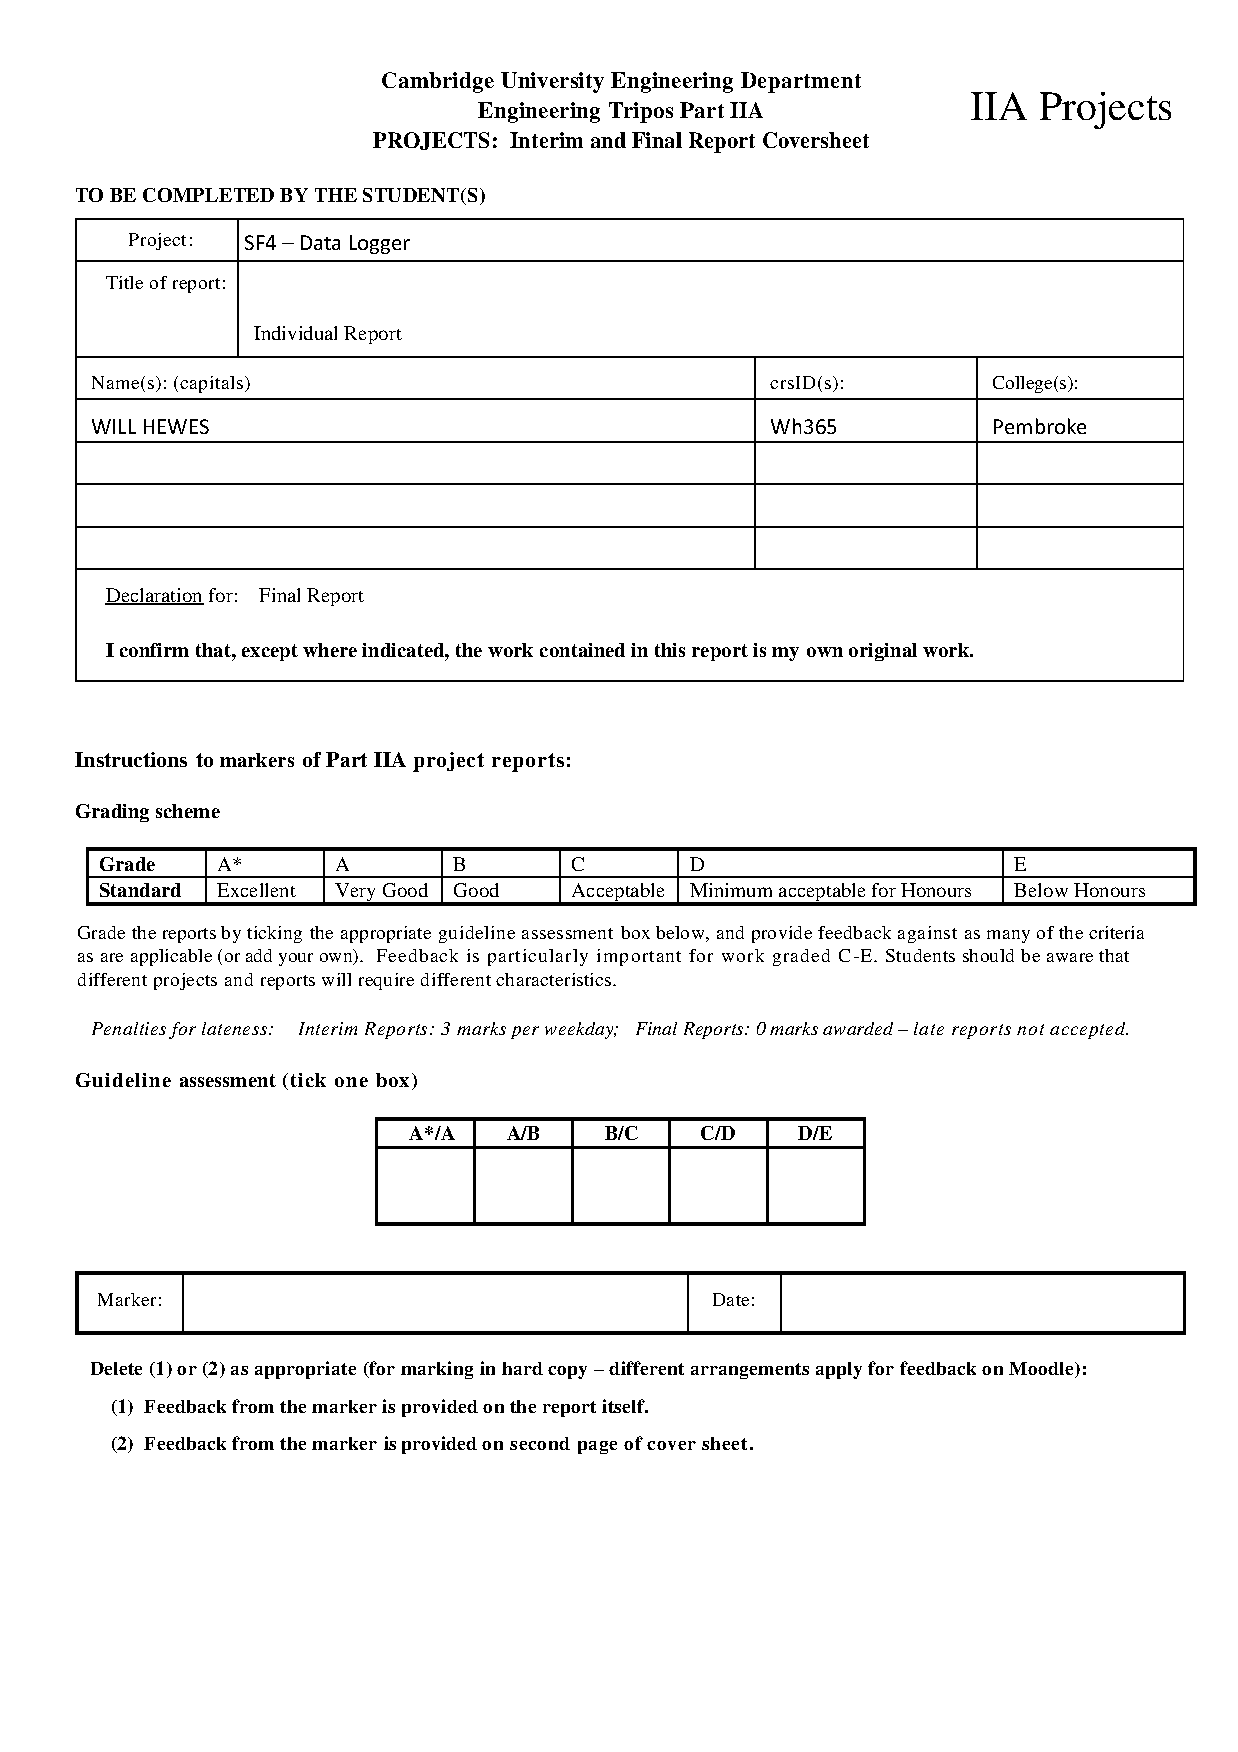
\includepdf[pages=-]{Handouts/IIA_Project_Coversheet Final Report.pdf}
\maketitle
\hrule
\tableofcontents
\newpage
\pagenumbering{arabic} \setcounter{page}{1}

\section{Introduction}
\label{sec:Introduction}

The aim of this project was to develop a microcontroller-based 
automatic plant watering system.
The system can autonomously monitor soil moisture levels, 
plot the data over time, and provide options to water the plant
manually when required or in response to threshold moisture levels.
This allows for effective monitoring and care with minimal user intervention.

In addition to moisture sensing, the system also tracks temperature, 
and was supposed to track humidity and light -
though this could not be implemented due to component delays.
This means most of the key factors affecting plant health
can be closely tracked, enabling detailed analysis of
optimum conditions for plant health.
These additional features enhance the system's utility
for control and research.

The motivation behind creating this autonomous watering system was twofold. 
Firstly, it can be used as demonstrated on a small scale,
allowing direct control over the conditions of one 
or a small number of houseplants,
offering a convenient way to care for plants.
This will remove the majority of the care required
to look after these often frail plants,
which is particularly useful over holidays or 
during the hot Summer months.
As a university student with several well-loved plants,
this has immediate personal appeal.

On a larger scale, the system provides a modular, 
low-cost framework adaptable to industrial or agricultural applications, 
where automated irrigation and environmental monitoring are increasingly valuable.
The low cost and simple design of the system will be appealing 
to large scale, versatile integration,
and the ease with which components can be added
and the GUI customised will allow for rapid expansion into the sector.

\section{Summary}
\label{sec:Summary}
% Summary of overall design decisions and outline of project management (1 side, possible team material)
\subsection{System Functionality}
% Describe at a high level what the system does

The system was designed to provide a robust, 
modular platform for automated plant watering, 
combining real-time environmental monitoring with servo-based actuation. 
At its core, the device reads soil moisture and temperature data, 
transmits this information via serial 
to a PC for logging and visualisation, 
and actuates a servo controlled pinch valve,
forming a water delivery mechanism.
This can be triggered manually when desired,
or in response to threshold values as typical operation. 
The system architecture was shaped by a clear division of responsibilities 
between microcontroller firmware and PC-based control logic, 
allowing for both immediate functionality and long-term extensibility.

\subsection{Project Management}
% Team roles, GitHub, modular workflow, timeline
\label{sec:PM}

\subsection{System Architecture}
% Arduino vs PC responsibilities, comms design, modularity, extensibility

\subsection{Hardware Selection}
% Sensors and actuators, with brief justification (no electrical detail)

From the outset, the project was developed collaboratively using GitHub, 
enabling effective version control and joint development across 
hardware, firmware, and software components. 
The project timeline was structured into three distinct phases: 
initial breadboarding and validation of individual components; 
development of communication infrastructure and 
GUI in parallel with firmware design; 
and full system integration and testing. 
A strong emphasis was placed on modular development, 
with sensors, control logic, and communication methods each validated 
independently prior to integration.

One early design choice was to simulate Arduino-PC communication 
using a socket-based protocol. 
This allowed rapid prototyping of the GUI and data parsing routines 
while the hardware was still under construction. 
This was essential in building the framework upon which the 
rest of the system could stand, 
including the setup of graphing capabilities,
the \textit{Serial Plotter} class,
and CSV handling capabilities.
Once physical components were ready, 
the system transitioned to serial USB communication, 
with the data format unchanged,
making for a straightforward development process.
Similarly, this modularity would now enable rapid upgrades to 
wireless communication protocols such as Bluetooth or Wi-Fi,
expanding the appeal and versatility of the product.

Responsibility for signal processing and decision-making was split 
across the two platforms. 
The Arduino handled low-level tasks, 
including sampling and averaging sensor values, 
applying basic calibration transformations, 
and formatting the data for serial transmission. 
It also listened for incoming commands to adjust the
threshold moisture values and the warning levels, as well as
being in control of all logic surrounding servo actuation,
which in turn controlled the flow of water from the reservoir. 
Meanwhile, the PC software performed higher-level tasks such as 
parsing the incoming data stream, logging time-stamped values to CSV files, 
and providing a user interface for threshold management and manual control.
Both systems were designed such that ...

Sensor and actuator selection was driven by 
practical constraints on budget, 
compatibility, and relevance to plant health. 
A capacitive soil moisture sensor was chosen for its long-term reliability 
compared to resistive alternatives,
as well as its fast response time and reliable signal acquisition. 

The temperature sensor (TMP36) provided a straightforward interface 
with adequate resolution and stability 
for environmental monitoring,
though some care had to be taken to ensure fluctuations and noise
did not interfere with its sensor data.
For this reason it also had a 100pF capacitor attached
between its signal and ground pins,
and the signal processing was eventually decided upon
primarily such that it would appropriately smooth out the 
sensors reported values 
while still allowing it to remain sufficiently responsive. 

The servo 

The servo-controlled water delivery mechanism was based on 
an open-source 3D-printed pinch valve, 
which offered simplicity and eliminated 
the need for complex pumping hardware. 

Additional sensors for light and humidity were ordered, 
but did not arrive in time for integration into the final build. 
Nonetheless, the system architecture remains extensible, 
with analogue and digital I/O capacity reserved for future expansion.

\begin{table}[H]
    \centering
    \renewcommand{\arraystretch}{1.5} 
    \makebox[\linewidth][c]{
    \resizebox{0.8\textwidth}{!}{
    \begin{tabular}{|c|c|c|}
        \hline
        \textbf{Order Code} & \textbf{Description of Component} & \textbf{Unit Price (£)} \\
        \hline
        2946124 & Capacitive Soil Moisture Sensor Module & 4.69 \\
        \hline
        SC21096 & Mini servo & 2.94 \\
        \hline
        4030054 & Temperature sensor & 1.38 \\
        \hline
        \rowcolor{yellow!60} 3167525 & Light sensor & 1.43 \\
        \hline
        \rowcolor{yellow!60} SN36746 & Humidity sensor & 0.91 \\
        \hline
        \multicolumn{2}{|c|}{\textbf{\large Total}} & \textbf{\large 11.35} \\
        \hline
    \end{tabular}
    }   
    }
    \caption{Component Order Summary}
    \label{tab:component_order}
\end{table}

\section{System Architecture}
\label{sec:System_Architecture}
% Include anmalogue circuitry, block diagram, and decision to include capacitors, lack of resistors etc.
% External power supply for servo

- block diagram\\
- description of general structure

\begin{figure}[H]
    \centering
    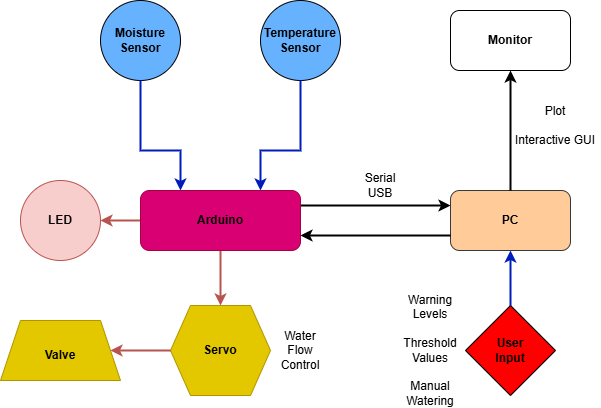
\includegraphics[width=0.8\textwidth]{Datalogger Block Diagram - final.png}
    \caption{Block Diagram for the automatic watering system}
    \label{fig:Block_Diagram_for_the_automatic_watering_system}
\end{figure}

\subsection{Circuit Design}
\label{Cicuit_Design}

- diagram\\
- testing sensors\\
- servo on seperate rail\\ 
- need for capacitors

\begin{figure}[H]
    \centering
    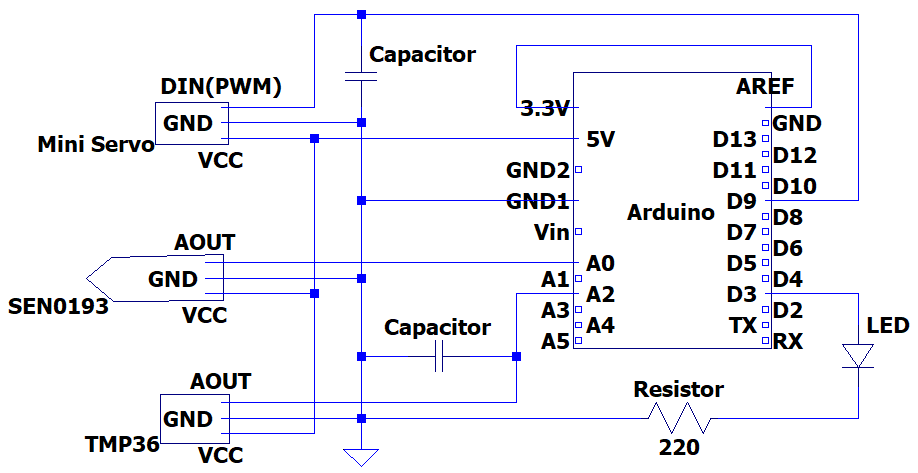
\includegraphics[width=0.8\textwidth]{Analogue Circuit Diagram - final.png}
    \caption{Analogue Circuit Diagram for the automatic watering system}
    \label{fig:Analogue_Circuit_Diagram_for_the_automatic_watering_system}
\end{figure}

\subsection{Watering System}
\label{sec:Watering_System}

- decision to use pinch valve\\
- necessity of reservoir sensor\\ 
- demonstration of components individually and collectively

\section{Code}
\label{sec:Code}
% Description of design/ computer code
\subsection{Firmware}
\label{sec:Firmware}
- sensors\\
- parsing, processing\\
- servo control

\subsection{Software}
\label{sec:Software}
- comms with Arduino\\
- GUI, plotting\\
- initial demonstration

\section{Technical Problemms}
\label{sec:Technical_Problems}
% Outline problems encountered in development and their technical solutions
- get Chengs help in drafting some interesting ones \\
- outline problem with powerrail if appropriate (not realising that these breadboards come with a gap in the powerrail)\\
- floating point problem for temp sensor

\section{Test Procedure}
\label{sec:Test_Procedure}
% Test procedure and software implementation
- testing individual compomnents one at a time \\
- testing the software presentation with a demonstration random data supply\\
- calibrating the moisture sensor with dry and with water\\
- determining the required servo rotation to elicit small quanmtiy of water\\
- use data from other sources to determine if humidity, light, and temp calibrated properly

\section{Further Improvements}
\label{sec:Further_Improvements}
- wifi module \\
- less jerryrigged water supply\\
- more sensors (CO2 conc)\\
- reservoir sensor\\
- greater control over parameters (mass of plant, type of plant)\\
- greater signal processing\\
- wider industrial applications

\subsection{Wider Industry}
\label{sec:Wider_Industry}
% Mention the watering systems currently being developed and the research undertaken
- deeper research into exact requirements\\
- close collaboration with farmers to set these requirements\\
- integrate a warning system to say that the specific conditions have been met (humidity requirements for harvesting etc, perhaps dangerous levels of heat)\\
- further integration of sensors, such as soil content (salt conc, fertiliser etc.)

\section{Conclusion}
\label{sec:Conclusion}

The aim of this project was to create a working demonstration of 
our autonomous watering system, with the ability to both log data
and dispense controlled quantities of water 
as the consumer dictates.
Overall, this has been a resounding success, 
acheiving the inital goal of moisture sensing and servo activation,
and expanding on this to include other senors 
and a more developed GUI.

The primary challenges and takeaways for a similar project in the future
include ...
Throughout this report it is evident that responsible practises 
such as detailed planning, modular testing,
and a feasible but expandable scope are integral to 
ensuring the success of a project like this.

This work could be expanded in the future to make a 
more sophisticated and professional datalogger
of the same scale,
incorporating more sensors, a more ... housing and 
general setup,
or could be further modified to be used in larger
industrial applications, such as informing agricultural farming
as is being researched by ...

\newpage
\appendix
\begin{thebibliography}{9}

\bibitem{arduino_servo}
Arduino. \textit{Servo Motor Basics with Arduino} : \\
\url{https://docs.arduino.cc/learn/electronics/servo-motors/}

\bibitem{tmp36}
Analog Devices. \textit{TMP35/TMP36/TMP37 Data Sheet} : \\
\url{https://www.analog.com/en/products/tmp36.html} 

\bibitem{arduino_tmp36}
ArduinoGetStarted. \textit{Arduino - TMP36 Temperature Sensor} : \\
\url{https://arduinogetstarted.com/tutorials/arduino-tmp36-temperature-sensor}

\bibitem{dfrobot}
DFRobot. \textit{Capacitive Soil Moisture Sensor SKU SEN0193} : \\
\url{https://wiki.dfrobot.com/Capacitive_Soil_Moisture_Sensor_SKU_SEN0193}

\bibitem{pinch_valve_design}
Printables. \textit{Pinch Valve Powered by Servo} : \\
\url{https://www.printables.com/model/247744-pinch-valve-powered-by-servo/files}

\end{thebibliography}

\section{Interim Report}
% 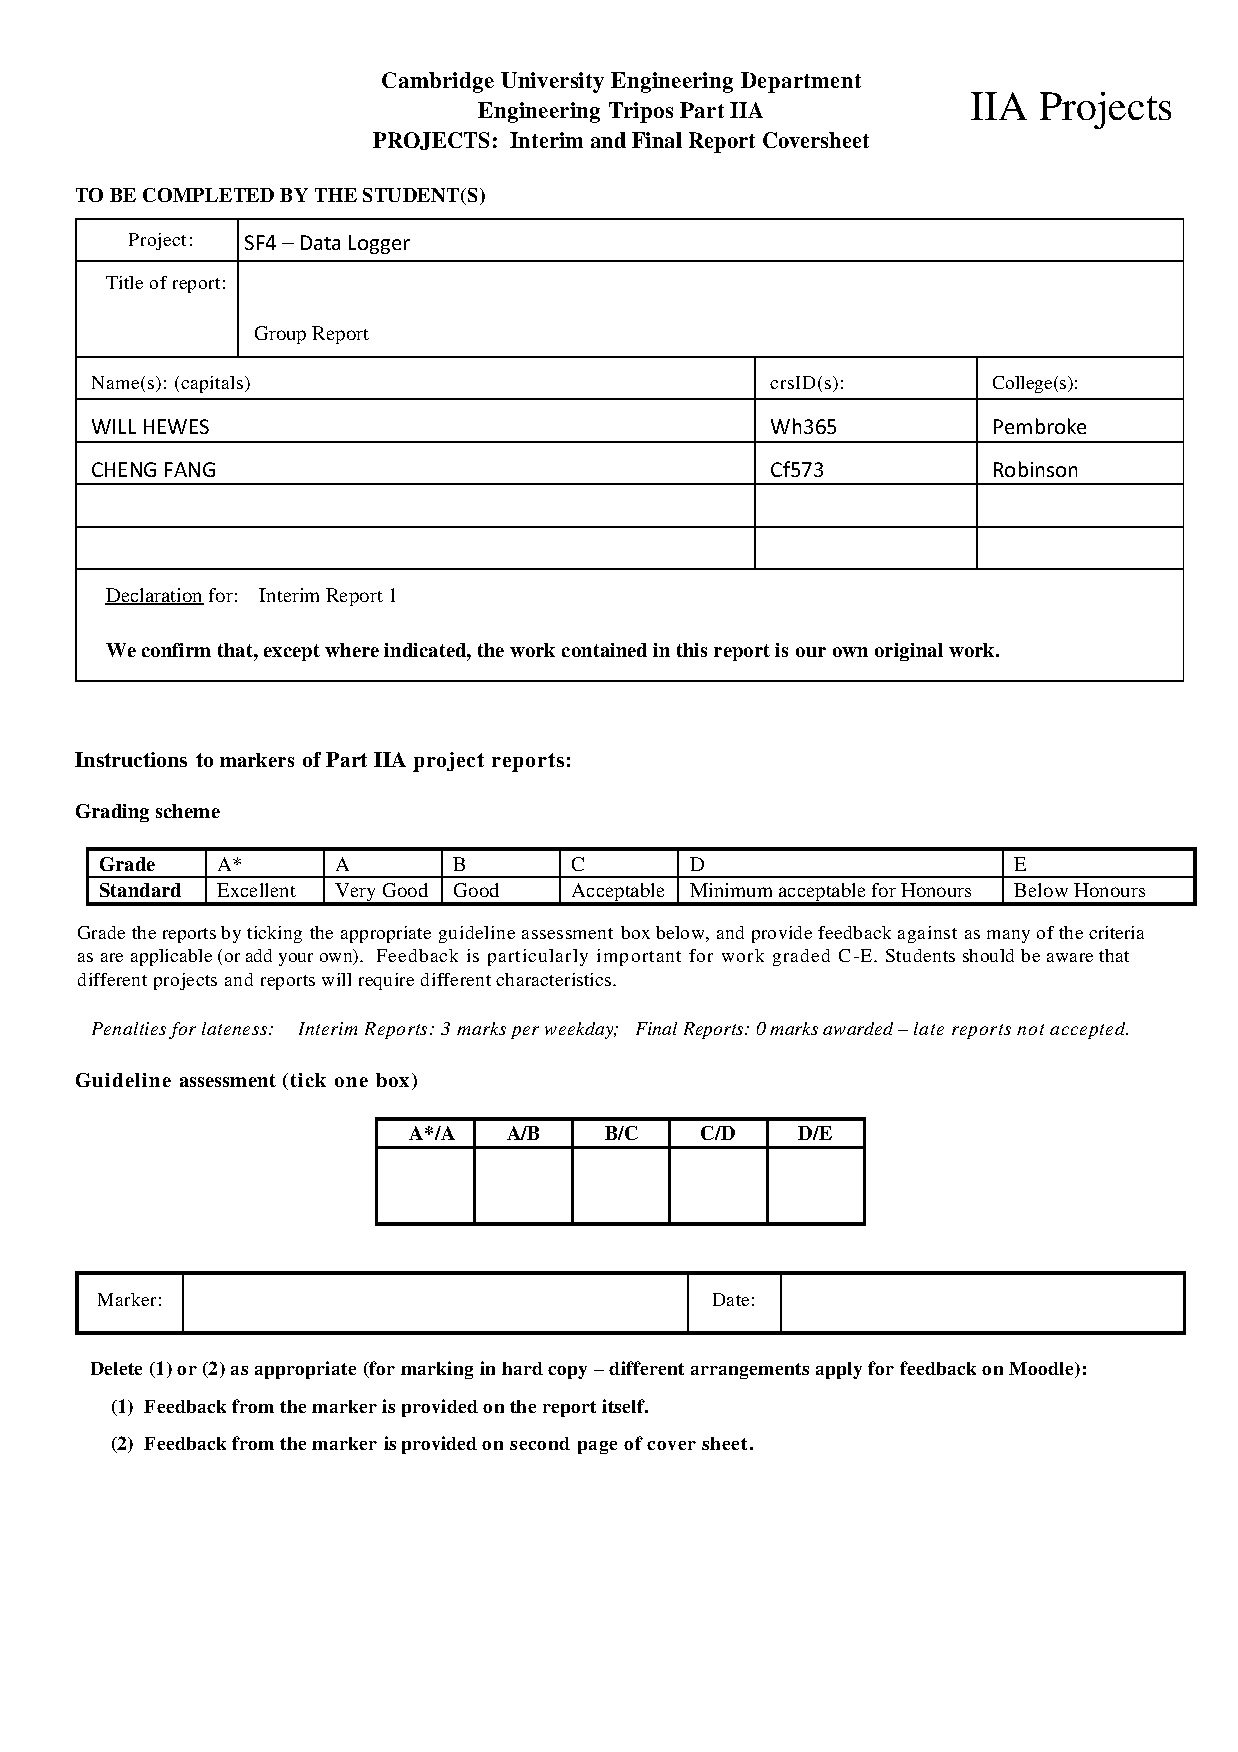
\includepdf[pages=-]{Reports/First Interim Report.pdf} % e.g. [pages={1,3-5,7}] to include pages 1,3,4,5,7
% Featuring the Interim Report

\end{document}